 
\section{Towards a ton-scale high-pressure xenon TPC.}

%%%%%%
\begin{figure}
\centering
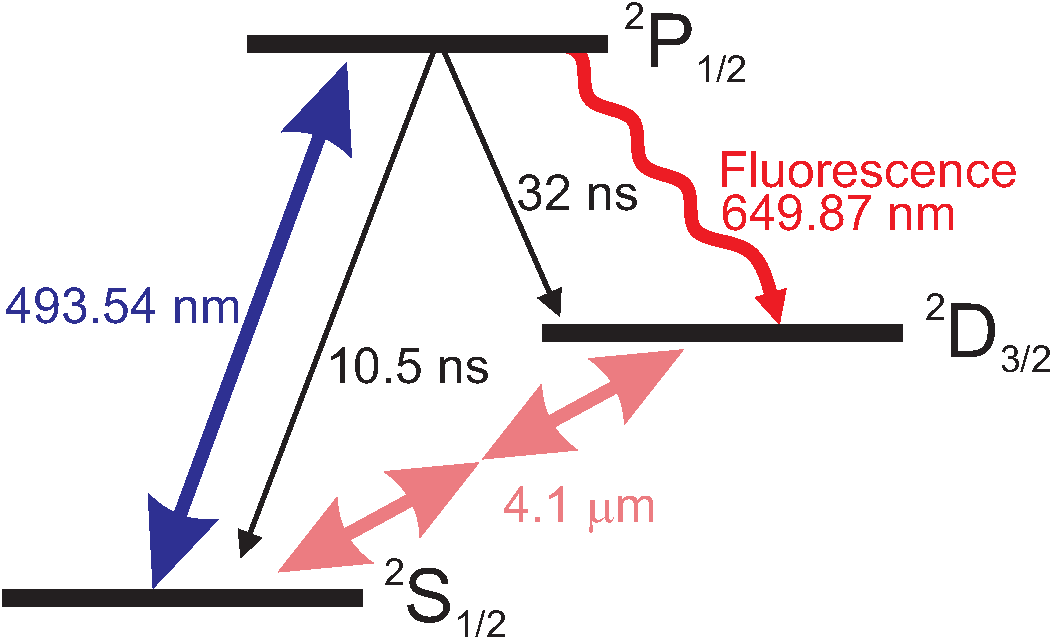
\includegraphics[width=0.60\textwidth]{img/levelscheme2.pdf}
\caption{\small The \BATA\ concept.} \label{fig.BATA}
\end{figure}
%%%%%%

If no discovery is made by the current generation of experiments, the full exploration of the CRR region (corresponding to the inverted hierarchy of neutrino masses, and \mbb\ values as low as 15~meV) requires detectors of larger mass (at least 1 ton), good resolution and extremely low specific background. The \HPXE\ technology has the potential to provide the most sensitive detector at this scale, by scaling the detector to a mass in the range of one ton and adding additional handles to further suppress the background. 


\subsection{Adding a magnetic field to enhance the topological signal}

%%%%%%%
\begin{figure}
\centering
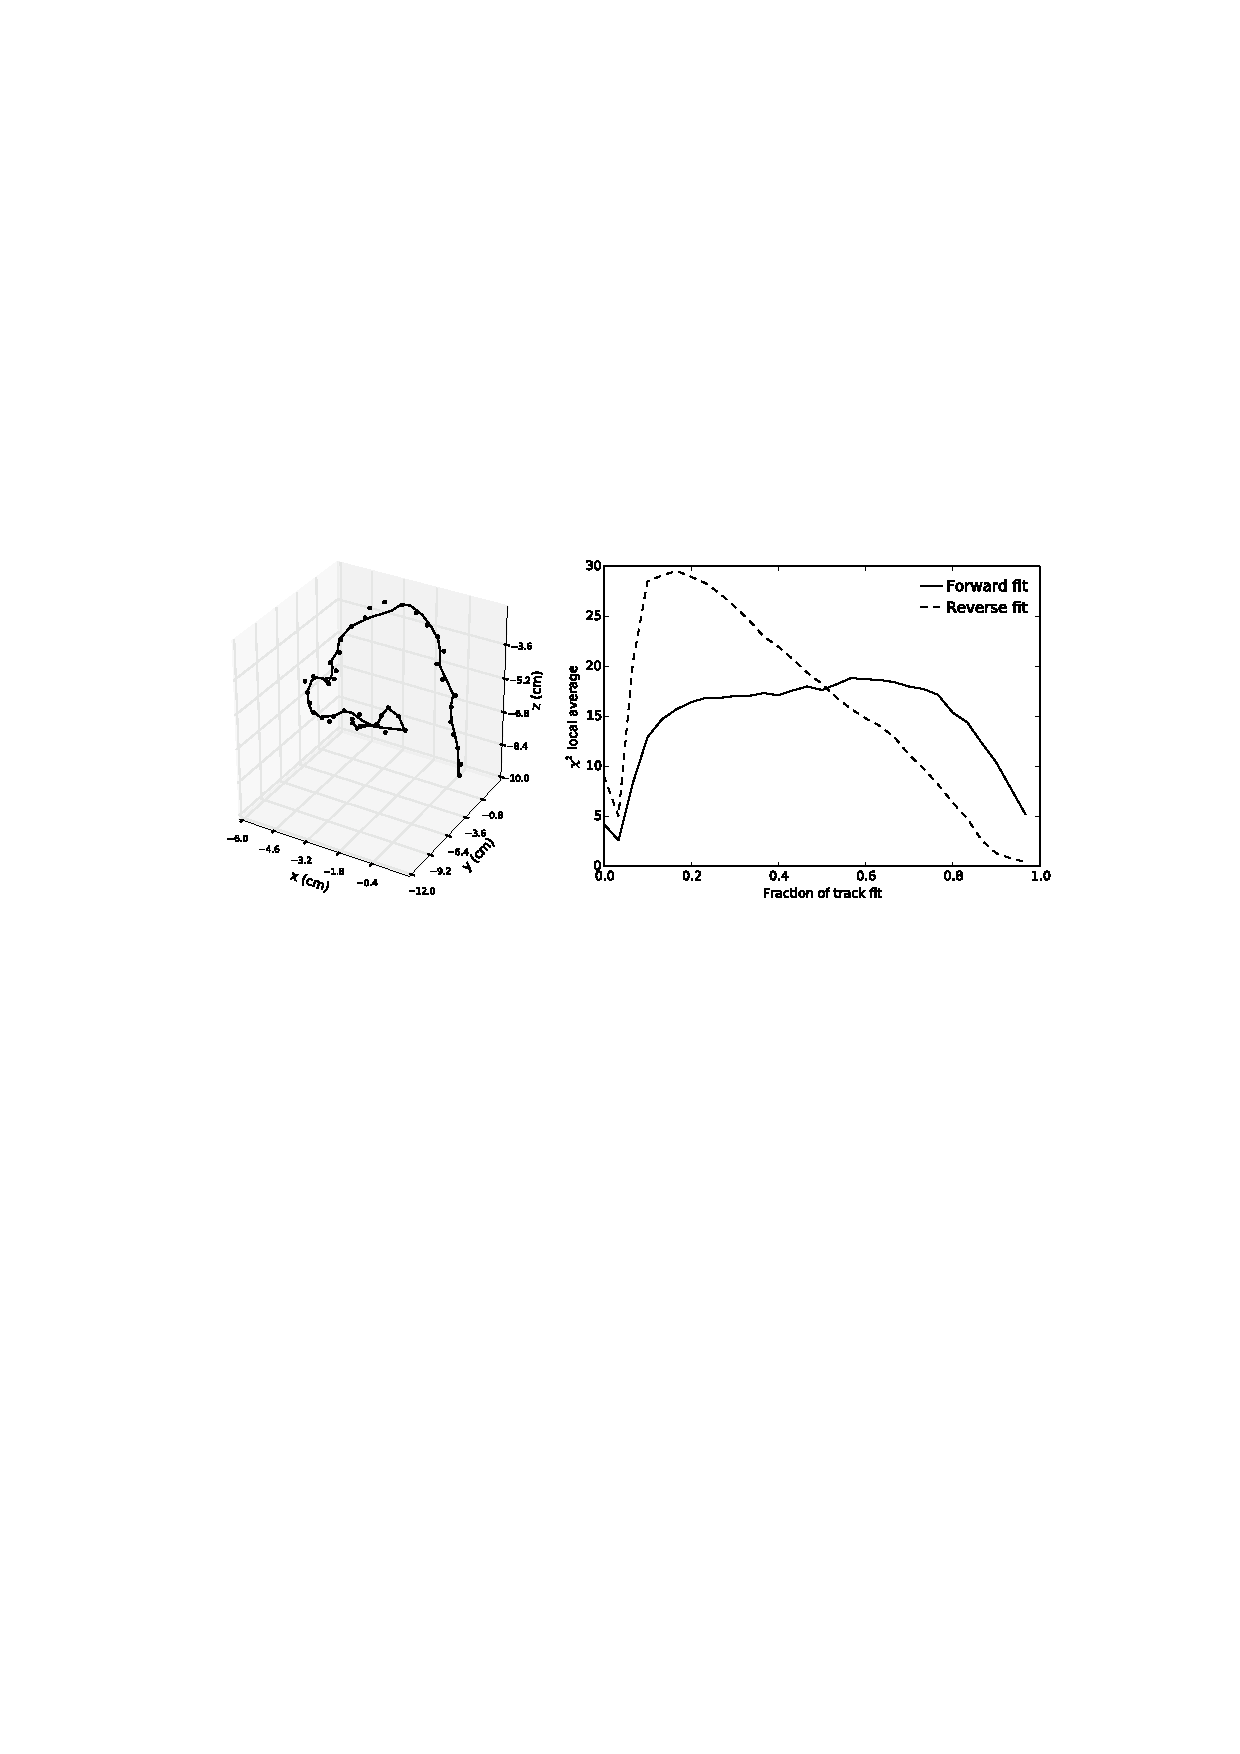
\includegraphics[width=0.99\textwidth]{img/KALMAN.pdf}
\caption{\small A Kalman Filter fit to a simulated (1 mm resolution) single-electron track in the proper direction of momentum flow. (Right) The local $\chi^2$ values produced along different points of the proper (``forward'') and improper (``reverse'') fits, averaged over $10^4$ single-electron tracks. Since the initial momentum is assumed to be the same in both fits, the $\chi^2$ value is artificially high at the beginning of the reverse fit (low multiple scattering error assumed, high multiple scattering found) and artificially low at the end (high multiple scattering error assumed, low multiple scattering found) .} \label{fig.KF}
\end{figure}
%%%%%%

The NEXT topological signal is based in the fact that single electrons (background events, produced by photoelectric and Compton interactions of high-energy gammas arising mostly from \BI\ and \TL) can be separated from double electrons (either \bbonu\ or \bbtnu) by the energy of the blobs defining the beginning and end of the track. As shown in Figure \ref{fig.ETRK2}, the energy of the blobs is roughly the same (and large), for signal events, while in background events, one of the blobs has an energy smaller than the other. We call this topological criterium of separating signal and background the {\bf blob signature}.

The physics mechanism behind the blob signature is energy deposition in the gas, which acts as a calorimeter. On the other hand, a second topological signature can be implemented by the addition of a moderate, uniform, magnetic field, $B= B_z$, pointing along the TPC axis. 

In the presence of such a field both of the emitted electrons in a $\bbonu$ (or a $\bbtnu$) decay, should spiral around the field lines in circular motion with radius $r = p_T/B$, where $p_T$~ is the momentum of the electron transverse to the direction of the field. A single energetic electron should produce a clear single spiral with radius indicative of its momentum, and a double-electron track with the same energy will produce two spirals each with much less momentum. This information provides an additional way of separating single-electrons arising from background processes from double electrons produced in \bb\ decays, {\bf in spite of the large multiple scattering that the electrons suffer in a dense \HPXE}.

An electron travelling through dense xenon gas undergoes several large-angle scatters that sharply divert an otherwise relatively smooth path through the detector. However, multiple scattering can be incorporated as a noise process, using (for example) the mathematical technique known as the Kalman Filter\footcite{Cervera:2002}. One can, then, perform fits to reconstructed electron tracks in both directions, {\bf assuming they are single-electron tracks with initial momentum corresponding to the kinetic energy released in $\bbonu$},  obtaining different results for single and double-electron tracks, as illustrated in Figure \ref{fig.KF}. For single-electron tracks, the fit should perform well in one direction (from the production vertex to the end vertex, since in this case the fit hypothesis is correct) and poorly in the other direction (from end vertex to production vertex, since now the hypothesis is totally wrong, and the electron has, as the start of the fit, vanishing momentum). For double-electron tracks, the fit should fail in both directions. 

The illustrative result displayed in Figure \ref{fig.KF}\footnote{J.J. Gomez-Cadenas, J. Renner, A. Cervera, J.A. Hernando, A. Imzaylov, F. Monrabal and J. Muñoz, ``Enhancing the topological signature of an HPXe detector by means of a magnetic field'', in preparation.} shows how the ``forward fit'' (from production to end vertex), differs from the ``reverse fit'' (from end vertex to production vertex), {\em even in the absence of a magnetic field}.  The right panel of the figure displays the local $\chi^2$~at each step of the fit. In the case of the forward fit (correct hypothesis), the fit converges rapidly to a flat value, since the Kalman Filter keeps updating the momentum of the electron as it losses energy by ionisation. Since the Kalman Filter model incorporates multiple scattering, the trajectory of the electron can indeed be followed, as shown in the left panel of the figure. Instead, the local $\chi^2$~for the reverse fit is too high at the beginning of the fit (the hypothesis is that the momentum is large, when in fact is is very small, therefore the predicted multiple scattering error is underestimated) and too small at the end of the fit (where the situation is reversed and thus the predicted multiple scattering error is overestimated).  

In the simulation, the assumed point-error is 1 mm. Such a resolution is difficult to achieve in NEXT-100, unless some additive to reduce the transverse diffusion is added. However, when a solenoidal magnetic field is added the E$\times$B effect reduces the lateral diffusion to negligible levels for any reasonable value of the field ($B=0.1$~Tesla is used for the simulations). In NEXT-100, position is reconstructed using SiPMs spaced at a pitch of 10 mm, yielding a resolution (if one would not make use of the SiPM recorded charge to weight the event position) of 3 mm, which improves to $\sim$~1 mm when the position is weighted by the SiPM recorded charge. Therefore, the resolution assumed in the plot is correct in the presence of a magnetic field (it could also be achieved adding suitable additives such as TMA). 

To further enhance the topological signature of NEXT (see Figure \ref{fig.ETRK2}), one performs a Kalman Fit to double-electron candidates (that is, those which have passed the selection cut requiring that the energy of the two blobs defining the beginning and end of the track is large). As noted, in true signal events, the momentum in each blob vanishes (each blob corresponds to the end-vertex of one of the two electrons emitted in a \bb\ decay). Instead, in background events managing to ``fake'' a blob at the start of the track, the fit will succeed in one direction (when we start from the fake blob, in which case the momentum is 2.3 MeV, corresponding to the kinetic energy of \Qbb), and will fail in the other (when we start from the true blob, where the momentum vanishes). Thus, fitting the candidates surviving the blob signature, {\em under the hypothesis that they are background electrons}, provide an extra rejection criteria. We fit the trajectory of the electron starting from both ends, and accept it only if the fit is consistent, in both cases, with a reverse fit.  This simple approach yields a factor 5 extra rejection (for 90\% signal efficiency), {\em in the absence of a magnetic field}.

Indeed, the rejection in the absence of magnetic field comes from an {\em indirect} measurement of the momentum of the electrons through their multiple scattering
angle $\theta_0$:

\begin{equation}
\theta_{0} = \frac{13.6}{\beta c p}\sqrt{\frac{x}{X_0}}+(1 + 0.038 \log{\frac{x}{X_0}})
\end{equation}
% 
 where $X_0$ is the radiation length of the dense xenon gas 
 $\sim P \times 8.48 ~g\cdot cm^{-2}$~where $P$~is the pressure of the gas) 
 $\beta c$~is the velocity of the electron and $p$~its momentum. 
 
 When a magnetic field $B$~ is added the (transverse) momentum of the electrons can be 
 directly measured,  $p_T = r \times B$. The determination of $p_T$ does not need to be accurate (which is fortunate, given the fact that the trajectory of the electrons is smeared by multiple scattering), because one relies in the strategy described above. Single (background) electrons will yield a good forward fit (where now the momentum of the electron must be consisted with the track curvature) and a bad reverse fit. Double (signal) electrons will yield reverse fits in two directions. Indeed, for candidate signal (double) electrons is is possible to scan the starting point of the reverse fit in both directions, until a good forward fit is found. This corresponds to the vertex of the double electron. We call the topological signature based in the measurement of the momentum of the track (either indirectly or with the aid of a magnetic field) the {\bf vertex signature}.
 
 Work is in progress to assess the final rejection factor and efficiency obtained when a magnetic field (of about $\sim$0.1 Tesla) is added and blob and vertex signatures are combined. Our preliminary studies indicate that the combination of both topological signatures will provide a factor of 10 extra rejection of backgrounds at little cost (90\%) 
 to the signal efficiency.  
 
 The current (estimated) rejection factor for NEXT-100 is 0.4 counts per ton and keV in a year. If a resolution of \Qbb\ of 0.5 \% FWHM is confirmed in the large detector as we expect, this translates into 5 counts per ton in the ROI. The addition of a magnetic field may yield a value of 0.5-1 counts per ton in the ROI, thus allowing the HPXe technology to operate in the ton regime without being background limited. 

\subsection{Barium Tagging}

As originally suggested by Moe\footnote{M.K. Moe, ``New approach to the detection of neutrinoless double-beta decay'', Physical Review C Rapid Communications 44 (1991) R931.}, a promising possibilities to further reduce the background is to develop the HPXe technology to unambiguously tag the barium ion produced in the xenon decay, $Xe \rightarrow Ba^{++} + 2 e^-$. The conceptual idea to tag $Ba^{+}$ is illustrated in Figure \ref{fig.BATA}. A ``blue'' laser of wavelength 493.54 nm excites (``pumps'') the S state, inducing $S \rightarrow P$~transitions, with a lifetime of $\sim$ 10 ns. About 30 \% of the times the \TwoP\ states decay to the state \TwoD, emitting ``red'' (649.76 nm) fluorescence in a characteristic time of 30 ns. The state \TwoD\ is metastable, but a second laser of suitable wavelength (4.1 $\mu$m) can be used to induce the transition to the ground state (this is known as ``deshelving'').  The whole cycle takes less than 50 ns, and therefore several millions of red fluorescence photons can be emitted by a single ion. 

The practical application of this conceptual idea is by no means easy, and in fact, it has been shown to be extremely difficult in liquid xenon by the work of the EXO collaboration\footcite{Dolinski:2012dta}. However, it may be feasible in a \HPXE\ detector, where a number of fortunate conditions may occur. These conditions are: a) charge reduction of the emitted barium ion, from $Ba^{++}$~to $Ba^{+}$, which can be induced by collisions with xenon atoms, or by the addition of a suitable quencher; b) ``trapping'' of the barium ion ``in situ'' by the surrounding Xe atoms, which result in a very low drift velocity for the ion; c) location of the ion, via the reconstruction of the event topology. 

All the above needs to be demonstrated with a systematic R\&D program, which must also address additional experimental issues such as pressure broadening of the laser, filtering of Rayleigh scattering, and others. The EXO collaboration has carried out extensive research of the potential for Barium Tagging, not only in a LXe TPC, but also in an \HPXE,\footcite{Sinclair:2011zz}. NEXT, on the other hand, has started a collaboration with CLPU\footcite{clpu}, a Spanish national facility dedicated to ultra-intense lasers, with the aim of carrying out a systematic R\&D program to understand the potential of Barium Tagging in a high pressure gas xenon TPC. Such a program
involves a set of proof-of-concept experiments, including:

\begin{enumerate}
	\item \textbf{Ba ions generation, phase 1}. Proof-of-principle experiment with Ba ions generated by means of an electrical discharge and/or laser ablation.
	
	\item \textbf{Ba ions generation, phase 2}. Proof-of-principle experiment with Ba ions generated by an ion source.	
		
	\item \textbf{D state deshelving}. A likely scenario is that the collisional induced decay between the metastable state D and the ground state S is either not effective or too slow for obtaining an appreciable fluorescence signal. In this situation the population is trapped in the metastable state D and the fluorescence cycle can not be closed. To avoid this difficulty, deshelving the D state may be needed. A proof-of-principle experiment with an additional laser for deshelving the D state will be performed. The laser needed must have a wavelength of around 4.1\,$\mu$m. The alternative, using a red laser would smear the characteristic red fluorescence with scattered photons from the deshelving laser.
\end{enumerate}

\subsubsection*{Proof of principle experiments}

In a first round of experiments we will excite resonantly the S$\leftrightarrow$P transition of {\bf Ba$^+$ ions generated by an electrical discharge} between two barium electrodes and will collect the fluorescence signal of the P$\rightarrow$D transition (alternatively, laser ablation can be used). Although this generation method is not ideal because several different species other than Ba ions will be generated (e.g., BaO molecules or clusters), it does not need a major technological development.

\begin{figure}
\begin{center}
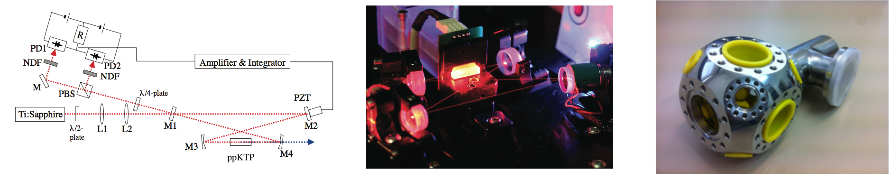
\includegraphics[width=0.99\textwidth]{img/blueLaser.png}
%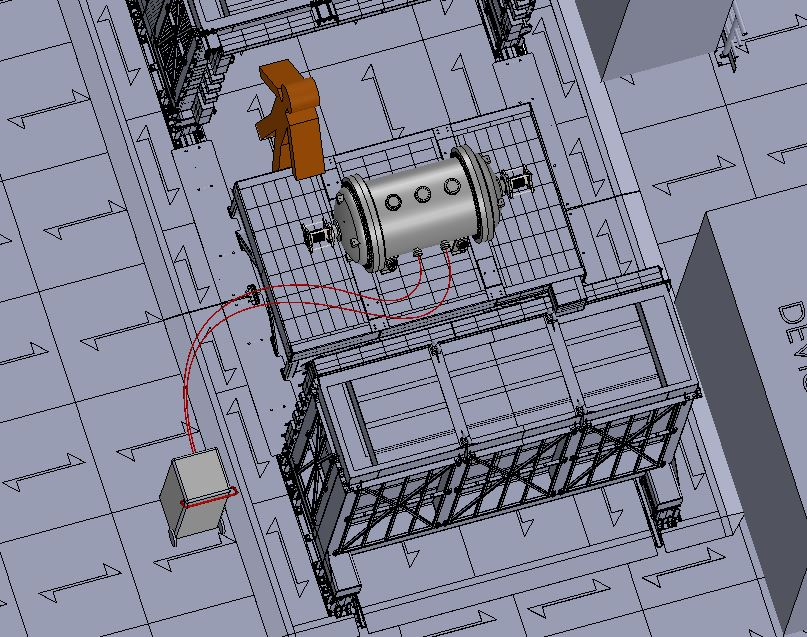
\includegraphics{img/CALIB_LSC_sources.jpg}
\caption{\small Left: experimental set-up for resonant frequency doubling of a 
Ti:Sapphire laser using ppKTP. Right: the chamber for the proof-of-concept experiments, built at IFIC, and ready to be installed at CLPU.}
\label{fig:chamber}
\end{center}
\end{figure}

The laser source needed to resonantly excite the $Ba^{+}$ ions must have a wavelength of 493.5\,nm, not available in commercial lasers. The laser source will therefore be produced at the CLPU, optimising a tunable Ti:sapphire laser at 987\,nm to obtain a second harmonic generation (SHG) at 493.5\,nm, see Figure \ref{fig:chamber}. This setup allows the tuning of the wavelength and the control of the bandwidth of the laser, a necessary feature to precisely tune it to the transition frequency (e.g. to correct for pressure broadening and other effects). Fig.~\ref{fig:chamber} also shows the test chamber needed for the experiments. 
We expect that this initial set of experiments will provide valuable information about the population dynamics in Ba$^+$ ions, and the influence of the different homogeneous and inhomogeneous broadening mechanisms. 

Next, we intent to generate Ba ions by an ion source that will be designed and constructed at the CLPU. This ion source will be based on selective ionisation and mass spectrometry techniques, and it will allow an efficient selection of the desired target species (e.g, $Ba^{+}$~and $Ba^{++}$). With this setup we will be able to study the recombination process Ba$^{++}\rightarrow$Ba$^{+}$ and decide whether it can be induced by collisions with xenon atoms, or whether it requires an additive (as demonstrated by ). Depending on the results of the experiment, a magnetic trap can be added to improve the experimental conditions. 

Finally, we intend to perform a proof of principle experiment with an {\bf additional laser for deshelving the D state}. Our approach will be to use a second laser to induce a two photon transition (one photon is forbidden by selection rules, between the states D and S, see Fig.\,\ref{fig.BATA}). 	

In our program we intend to reproduce and extent the pioneer work of Sinclair and others\footcite{Sinclair:2011zz}, in particular focusing in the scenario of barium-tagging ``in situ'' (the approach of the EXO R\&D appears to be to extract the barium ion, both in the case of liquid and gas detectors). In any case, we believe that the barium tagging program offers a opportunity of joint development with the EXO collaboration.

Clearly the construction of a ton-scale \HPXE\ detector implementing the full Barium Tagging technology is a very challenging enterprise. On the other hand, it appears to be a promising path towards the future. 


  
\subsection{NEXT will be BEXT}
The addition of either a B-field or Barium Tagging (or both), are clear forward paths to improve the NEXT detector towards the future BEXT\footnote{B-field Experiment with a Xenon TPC, also Barium-Taggin Experiment with a Xenon TPC} apparatus, displaying  
a mass in the range of several tons, with a resolution of 0.5 \% FWHM and a background rate in the range of $10^{-4}$ (this appears relatively easy to achieve with a magnetic field) to $10^{-6}$ (as ultimately possible with barium-tagging) \ckky\ would be able to fully cover the CRR (and inverted hierarchy) region event in the most pessimistic NME scenario. 



